\documentclass[a4paper,12pt]{article}

\usepackage[utf8]{inputenc}
\usepackage[czech]{babel}
\usepackage[IL2]{fontenc}
\usepackage[left=3cm,text={15cm, 23cm},top=3.5cm]{geometry}

\usepackage[dvipdf]{graphicx}

\bibliographystyle{czplain}

\def\author{Vojtěch Havlena (xhavle03)\\ & Karel Březina (xbrezi13)}
\def\projname{Téma 6: Plynová krize v Evropě}

\begin{document}

  \begin{titlepage}

% \vspace*{1cm}
\begin{figure}[!h]
  \centering
  \includegraphics[height=5cm]{img/logo.eps}
\end{figure}

\vfill

\begin{center}
  \bigskip
  \begin{Huge}
  \projname\\
  \end{Huge}
  \begin{large}
  Simulační studie k projektu do předmětu IMS\\
  \end{large}
\end{center}

\vfill

\begin{center}
  \begin{Large}
  \today
  \end{Large}
\end{center}

\vfill

\begin{flushleft}
\begin{large}
\begin{tabular}{ll}
Autor: & \author \\
 & Fakulta Informačních Technologií \\
 & Vysoké Učení Technické v~Brně \\
\end{tabular}
\end{large}
\end{flushleft}
\end{titlepage}

  
  \tableofcontents
  
  \newpage
  % ---------------------------------------------------------------------------
  % Úvod
  % ---------------------------------------------------------------------------
  \section{Úvod}
  Tato práce vznikla v rámci projektu do předmětu Modelování a simulace. V práci 
  je řešena simulace (\cite{peringer}, slide 8) modelu (\cite{peringer}, slide 7) spotřeby a produkce plynu ve vybraných 
  Evropských státech. Na základě modelu a simulačních experimentů je zjišťována 
  dostupnost plynu v jednotlivých státech za daných krizových situací. Smyslem 
  dílčích experimentů je ukázat různé alternativy řešení dané krizové situace.
  
  \subsection{Autoři a zdroje informací}
  Autory práce jsou Vojtěch Havlena a Karel Březina. Mezi hlavní zdroj informací 
  lze zařadit mapy a další data z webových stránek Gas Infrastructure Europe \-
  (\texttt{http://transparency.gie.eu/}). Další 
  potřebné informace byly zjišťovány z webových stránek národních dodavatelů plynu 
  v jednotlivých zemích.
  
  \subsection{Experimentální ověření validity}
  Experimentální ověření validity modelu (\cite{peringer}, slide 37) probíhalo na základě porovnávání zjištěných 
  reálných hodnot stavu zásobníků plynu v jednotlivých státech s výsledky experimentu, 
  ve kterém se simulovalo dodávání plynu podle reality.
  
  Pokud porovnáme výsledek experimentu s grafy, které jsou volně dostupné na  
  \texttt{http://transparency.gie.eu/}, lze zjistit, 
  že půběhy grafů jsou mezi sebou korelovány.
  
  \begin{figure}[!ht]
    \centering
    \includegraphics[height=7cm]{img/val.eps}
    \caption{Výsledek experimentu zjišťující množství plynu v zásobnících jednotlivých států 
    během roku. Nejsou uvažovány plánované LNG terminály. Z důvodu čitelnosti grafu zde není zobrazeno Rusko.}
  \end{figure}
  
  Rozdíly mezi maximálními a minimálními hodnotami plynu v zásobnících jednotlivých států
  \footnote{Jsou uvedeny pouze státy, jejichž hodnota kapacity zásobníků během časového období se podařila zjistit.} lze shrnout následující tabulkou:
  
  \begin{table}[h!]
  \centering
  \begin{tabular}{| l | l | l |}
    \hline
    \textbf{Stát} & \textbf{Výsledek experimentu} & \textbf{Zjištěná hodnota} \\
    & [mil. m$^3$] & [mil. m$^3$] \\
    \hline\hline
    Česká republika & 1371 & 1440 \\ \hline
    Polsko & 1267 & 1088 \\ \hline
    Maďarsko & 1839 & 1712 \\ \hline
    Německo & 12520 & 14877 \\ \hline
    Slovensko & 997 &  1284 \\
    \hline
  \end{tabular}
  \caption{Rozdíly mezi maximálním a minimálním objemem plynu v zásobnících jednotlivých států během roku.}
  \end{table}
  
  \section{Rozbor tématu a použitých metod/technologií}
  Každý stát obsahuje několik zásobníků pro uložení plynu. Spotřeba plynu každého státu se liší podle ročního období. 
  Poměr letní a zimní spotřeby se nepodařilo zjistit pro Bělorusko a Rusko, avšak podle polohy těchto států a 
  hodnot zjištěných u ostatních států jsme tento poměr odhadli (tabulka~\ref{tab2}) \cite{mapa1}.
  
  Kvůli maximální živostnosti plynovodů se objem dodávek plynu během roku mění jen minimálně. Plynové zásobníky 
  jednotlivých států slouží právě k vyrovnání tohoto rozdílu mezi dodávkou a spotřebou. Některé státy disponují 
  také vlastní produkcí plynu. Některé státy taktéž exportují plyn do okolních států. Mezi jednotlivými státy 
  je plyn rozváděn pomocí plynovodů. Každý plynovod je určen maximální průtokovou kapacitou v jednotce množství 
  za hodinu. Rychlost plynu se pohybuje až kolem 40 km/h \cite{speed}.
  
  Mezi hlavní dodavatele plynu v Evropě patří Rusko a Norsko. Plyn z Ruska proudí do centrální Evropy přes 
  plynovod Yamal (přes Bělorusko do Polska), Nordstream (podmořský plynovod do Německa) a plynovod Družba 
  (přes Ukrajinu, Slovensko do České republiky). Plyn z Norska proudí přes plynovody Europipe I a Europipe II 
  z přístavních LNG terminálů Kollsnes 1+2 \cite{kollsnes} a Snurrevarden do Německa. Souhrn zjištěných informací o plynovodech 
  spojující jednolivé státy lze nalézt v tabulce~\ref{tab4}. Mezi další LNG terminály, které dodávají 
  plyn do uvažovaných zemí patří Belgické Zeebrugge \cite{zeebrugge} a Nizozemský Rotterdam \cite{rotterdam}. 
  Posledně zmiňované dodávají plyn do Německa (kapacita LNG terminálů -- tabulka~\ref{tab3}).
  
  Nicméně v budoucnu by se měli otevřít další LNG terminály, které mohou ovlivnit závislost na ruském plynu. Mezi 
  nejdůležitější patří pravděpodobně budovaný polský terminál Swinoujscie a chorvatský teminál Adria \cite{prouza}. Tyto terminály 
  by měli být spojeny Severojižním koridorem, přes Polsko, ČR, Slovensko, Maďarsko a Chorvatsko. Je plánována také 
  výstavba LNG termínálu pro dovoz z USA, ale o něm neexistuje zatím moc konkrétních informací. Proto jsme kapacitu a 
  umístění terminálu zvolili podle našeho uvážení a podle útržkovitých nalezených informací \cite{usa}.
  
  Zjištěné informace jsou shrnuty v následující tabulce.
  
  \begin{table}[h!]
  \centering
  \begin{tabular}{| l | l | l | l | l |}
    \hline
    \textbf{Stát} & \textbf{Spotřeba} & \textbf{Produkce} & \textbf{Kapacita zás.} & \textbf{Koef. letní}  \\ 
     & [tis. m$^3$/h] & [tis. m$^3$/h] & [tis. m$^3$] & \textbf{spotřeby} \\
    \hline\hline
    Česká republika & 968 & 29 & 3436000 & 0.639 \\ \hline
    Polsko & 2081 & 709 & 2524000 & 0.805 \\ \hline
    Maďarsko & 1041 & 222 & 6330000 & 0.557 \\ \hline
    Německo & 10096 & 1345 & 22027000 & 0.78 \\ \hline
    Slovensko & 664 & 0  & 3020000 & 0.637 \\ \hline
    Ukrajina & 5875 & 2288 & 31950000 & 0.798 \\ \hline
    Bělorusko & 2338 & 27 & 2832000 & 0.820 \\ \hline
    Rusko & 53289 & 76584 & 70400000 & 0.812 \\
    \hline
  \end{tabular}
  \caption{Spotřeba, produkce a kapacita zásobníků sledovaných států z roku 2013 (zdroj: \cite{info}). Sloupec koeficient letní spotřeby udává 
  hodnotu $p$, kterou se násobí průměrná spotřeba v létě. V zimním období se průměrná 
  spotřeba násobí hodnotou $2-p$. (zdroj: spočítáno z \cite{mapa1}) }
  \label{tab2}
  \end{table}
  
  \begin{table}[h!]
  \centering
  \begin{tabular}{| l | l |}
    \hline
    \textbf{LNG terminál} & \textbf{Kapacita}  \\
     & [tis. m$^3$/h] \\
    \hline\hline
    Kollsnes & 5958 \\ \hline
    Snurrevarden & 3208 \\ \hline
    Rotterdam & 1369  \\ \hline
    Zeebrugge & 1027 \\ \hline
    Swinoujscie & 854 \\ \hline
    Adria & 1708 \\ \hline
    USA & 6500 \\
    \hline
  \end{tabular}
  \caption{Kapacita LNG terminálů (zdroje: \cite{prouza}, \cite{usa}, \cite{rotterdam}, \cite{zeebrugge})}
  \label{tab3}
  \end{table}
  
  \begin{table}[h!]
  \centering
  \begin{tabular}{| l | l | l | l |}
    \hline
    \textbf{Plynovod} & \textbf{Kapacita} & \textbf{Délka} & \textbf{Přepr. doba}  \\
     & [tis. m$^3$/h] & [km] & [h] \\
    \hline\hline
    Rusko -- Ukrajina & 8542 & 775 & 19  \\ \hline
    Ukrajina -- Slovensko & 8542 & 1010 & 24 \\ \hline
    Bělorusko -- Polsko & 3843 & 480 & 12 \\ \hline
    Rusko -- Bělorusko & 3843 & 695 & 17 \\ \hline
    Ukrajina -- Maďarsko & 2232 & 905 & 22 \\ \hline
    Ukrajina -- Polsko & 509 & 691 & 17 \\ \hline
    Rusko -- Něměcko & 6539 & 1222 & 30 \\ \hline
    Slovensko -- ČR & 1978 & 300 & 7 \\ \hline
    Maďarsko -- Slovensko & 1640 & 165 & 4 \\ \hline
    ČR -- Polsko & 104 & 525 & 13 \\ \hline
    Německo -- Polsko & 1942 & 517 & 12 \\ \hline
    Německo -- ČR & 1197 & 285 & 7 \\ \hline
    Kollsnes 1+2 -- Německo & 1916 & 670 & 16 \\ \hline
    Snurrevarden -- Německo & 2958 & 670 & 16 \\ \hline
    Zeebrugge -- Německo & 1655 & 590 & 14 \\ \hline
    Rotterdam -- Německo & 1655 & 609 & 15 \\ \hline
    Swinoujscie -- Polsko & 1640 & 100 & 2 \\ \hline
    Adria -- Maďarsko & 1640 & 359 & 8 \\ \hline
    USA -- Polsko & 3000 & 100 & 2 \\
    \hline
  \end{tabular}
  \caption{Maximální kapacita plynovodů (zdroj: \cite{mapa2}, spočítáno pomocí nástroje dostupného na: 
  \texttt{http://www.interconnector.com/units-converter}). Přepravní doba byla spočítána jako podíl 
  délky plynovodu a rychlosti plynu (40 km/h).}
  \label{tab4}
  \end{table}
  
  \subsection{Použité postupy}
  Pro implementaci byl zvolen jazyk C++, taktéž kvůli podpoře objektově orientovaného programování, 
  které se pro řešení hodí. Nakonec jsme se rozhodli nepoužít knihovnu SIMLIB, protože v 
  projektu simulujeme pohyb velkého množství plynu a to by použítí této knihovny komplikovalo. Pro vykreslení 
  grafů je použit volně dostupný nástroj gnuplot, který je dostupný na \texttt{http://www.gnuplot.info/}.
  
  \section{Koncepce}
  V systému, jak již bylo zmíněno dříve, se vyskytují státy. Oproti zadání jsme si seznam sledovaných 
  států rozšířili o Bělorusko a Německo. Každý stát obsahuje zásobník plynu s určitou kapacitou. 
  Zásobníky lze chápat jako sklady s danou kapacitou.
  Odtud se bere plyn pro pokrytí spotřeby daného státu. Uvažujeme, že spotřeba se pohybuje v náhodném 
  rozmezí $\pm 10 \%$ od průměrné spotřeby v ročním období daného státu. Roční období léto a zima se 
  střídá vždy po 6 měsících. Státy mohou být připojeny k výstupním plynovodům, 
  kudy posílají plyn jednotlivým státům. O tom, jaké množství plynu státy pošlou rozhoduje použitá strategie. 
  V našem případě se jedná o \uv{hladovou} strategii. Množství exportovaného plynu je dáno následujícím vzorcem:
  $$
    p_{exp} = \max\{ p_{imp} - p_{cons} + p_{prod}, 0 \}, 
  $$
  kde $p_{exp}$ je množství exportovaného plynu, $p_{imp}$ je mn. importovaného plynu a $p_{cons}$ resp. 
  $p_{prod}$ je spotřeba plynu resp. produkce daného státu. Uvedená strategie znamená, že státy se v první 
  řadě snaží pokrýt svoji spotřebu a exportují až zbytek. Exportovaný plyn se posléze rozdělí podle poměru 
  kapacit výsledných plynovodů. Pro účely validace modelu byla vytvořena i \uv{smluvní} strategie. V ní je 
  odesílané množství plynu předem známo, tato strategie se však příliž nehodí pro simulaci krizových situací, 
  proto nebude dále uvažována. 
  
  LNG terminály jsou modelovány jako zásobníky plynu. V modelu předpokládáme, že po každé hodině dojde k 
  doplnění až do maximální kapacity plynu (o způsobu doplňování plynu nebylo nalezeno dostačné množství 
  relevantních informací).  
  
  Posledním modelovaným prvkem systému jsou plynovody. Charakteristikou plynovodu je maximální množství 
  plynu za hodinu, které je možné přes něj přenést (pouze v jednom daném směru). V případě, že se nějaký stát rozhodne poslat určité 
  množství plynu přes plynovod, do druhého státu množství plynu dorazí za dobu danou podílem délky 
  plynovodu a rychlostí plynu. Délku u plynovodů ležících na pevnině uvažujeme jako vzdálenost mezi 
  hlavními městy států, které plynovod spojuje. Opět z důvodu nedostatku relevantních informací, rychlost 
  přenášeného plynu uvažujeme jako konstantu. Toto zjednodušení má za následek pouze větší prodlevu při 
  doručení plynu.
  
  \subsection{Způsob vyjádření konceptuálního modelu}
  Pro účely vyjádření konceptuálního modelu je zvolena kombinace slovního popisu uvedeného výše a grafického popisu 
  sítě plynovodů mezi jednotlivými uzly (obrázek 2). Částečný popis pomocí petriho sítě je sice možný, ale ne úplně 
  smysluplný. 
  
  \subsection{Forma konceptuálního modelu}
  \begin{figure}[!ht]
    \centering
    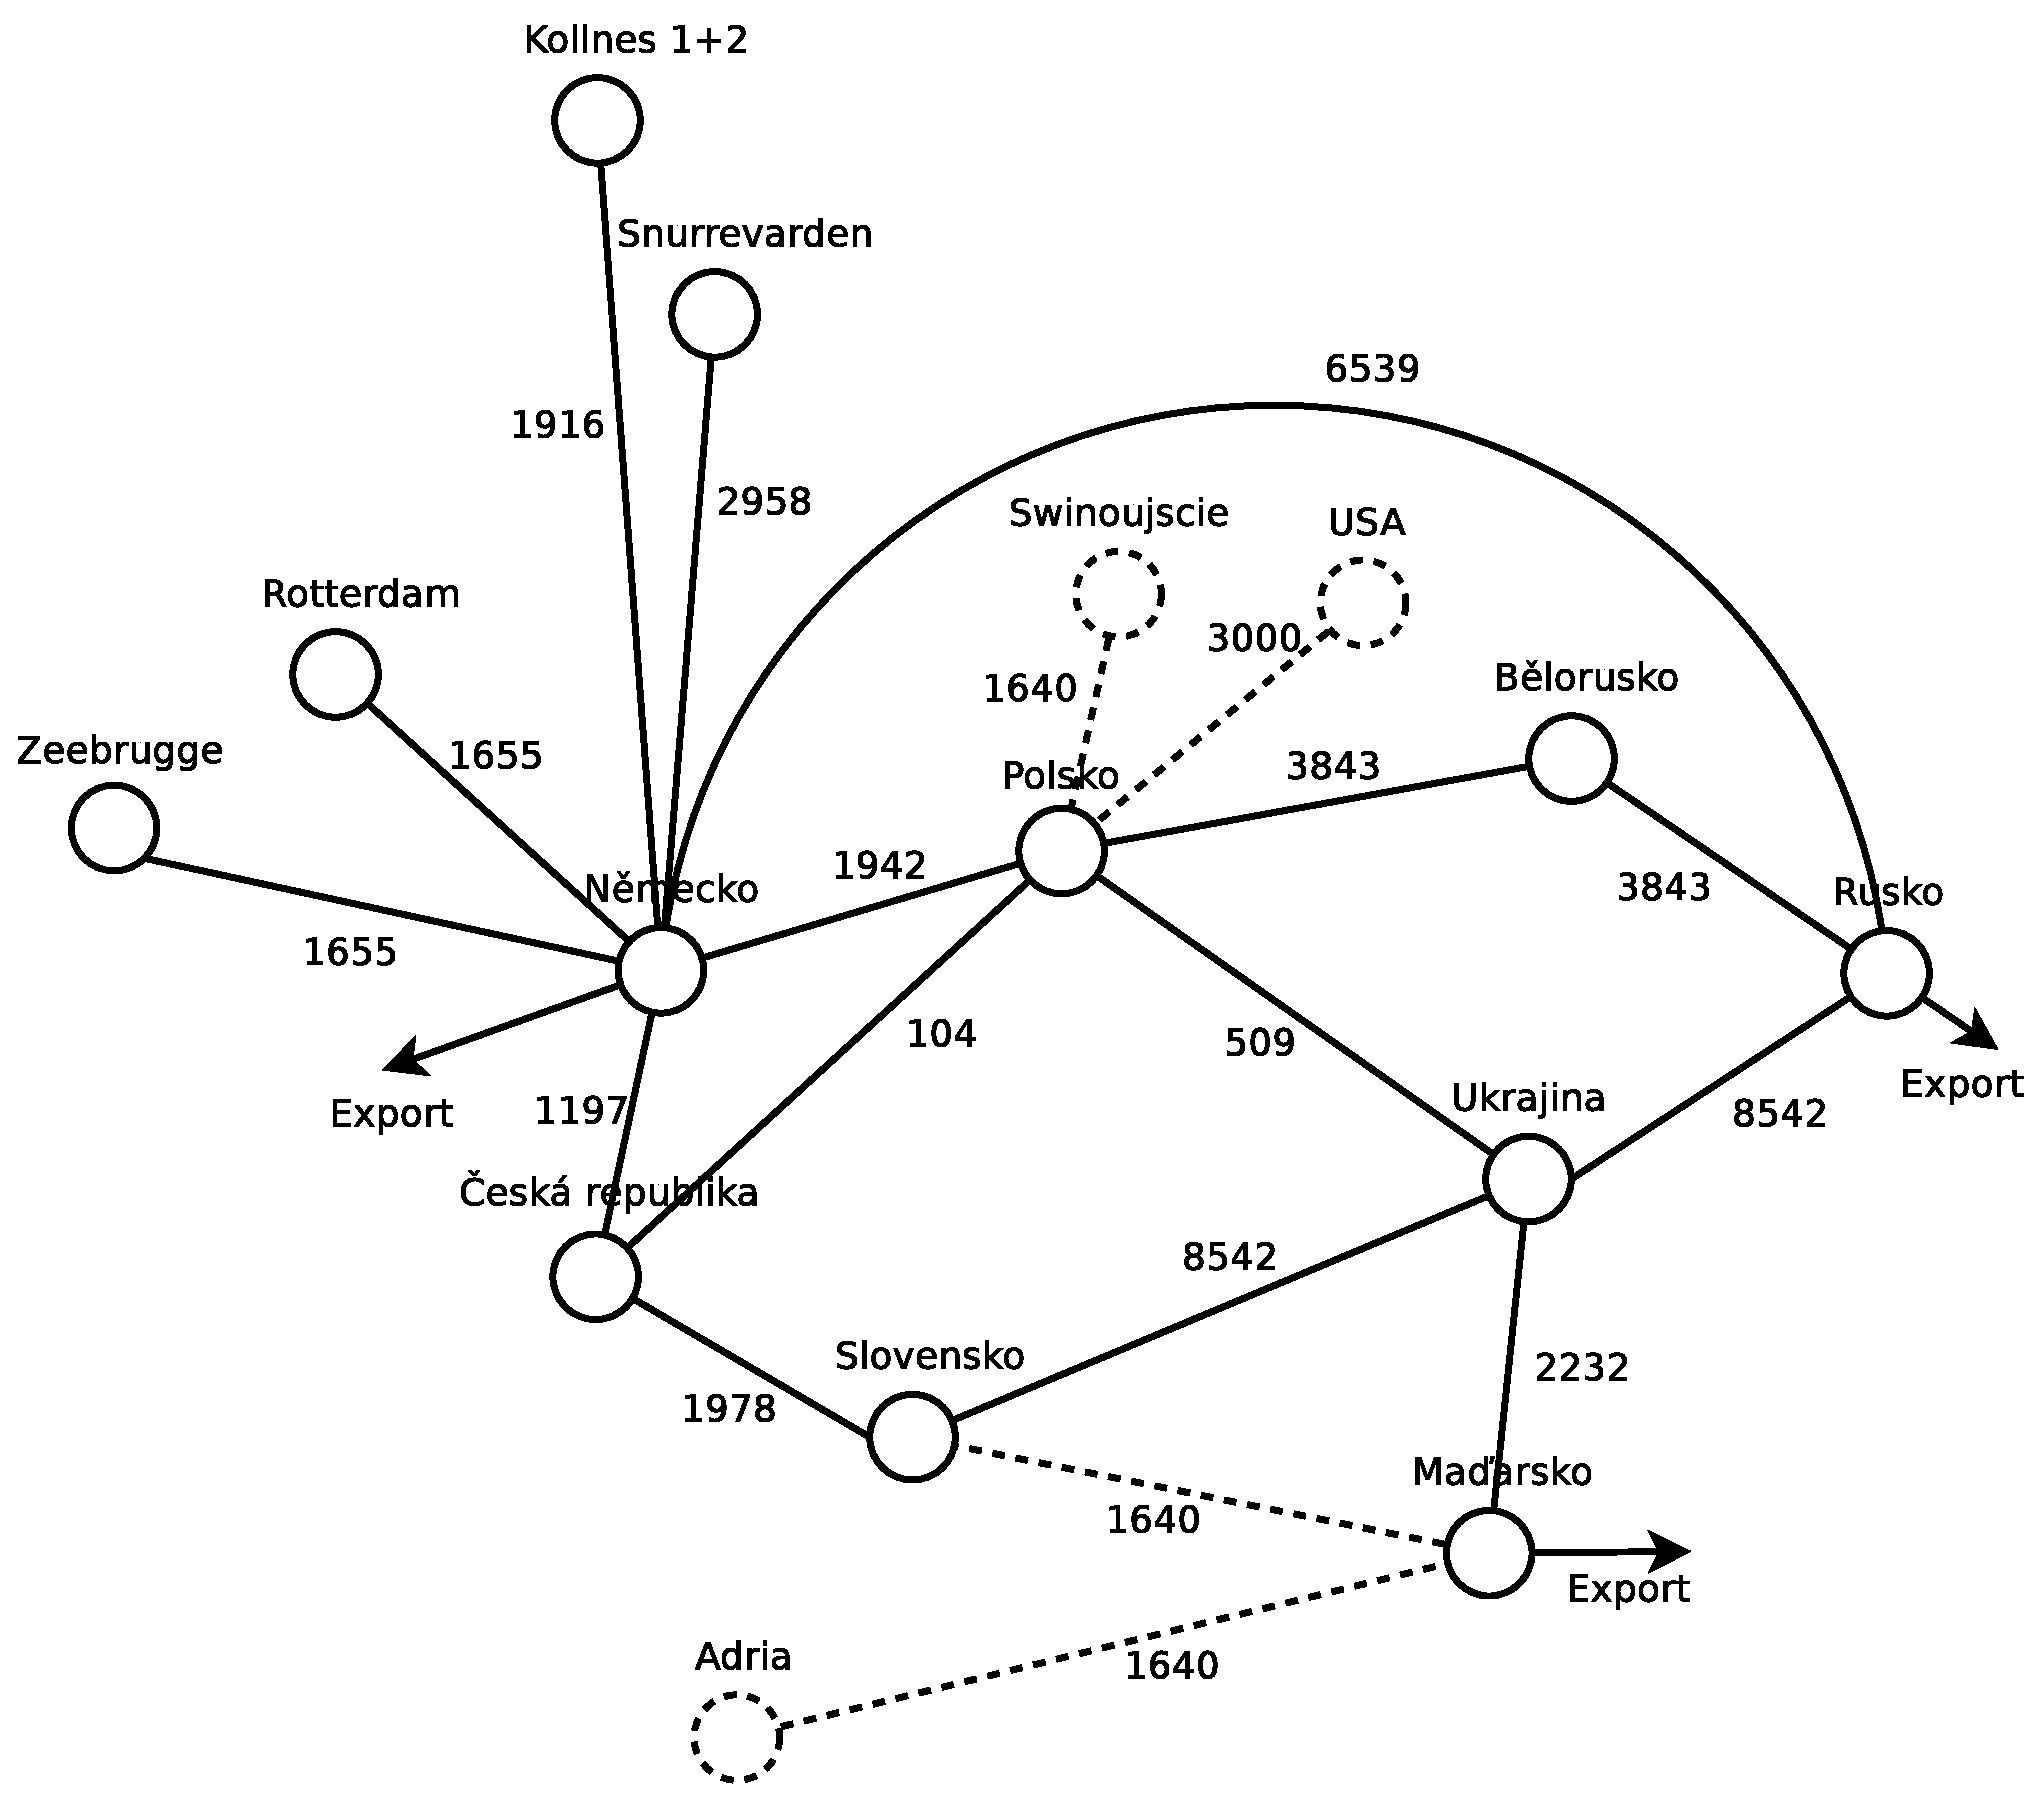
\includegraphics[height=12.5cm]{img/model.eps}
    \caption{Popis sítě plynovodů s uvažovanými státy a LNG terminály. 
    Tečkovaně jsou uvedeny plánované plynovody a LNG terminály. Ohodnocení hran udává maximální přenosovou kapacitu plynovodu v $m^3/h$.}
  \end{figure}
  
  \section{Architektura simulačního modelu/simulátoru}
  Jak již bylo zmíněno v podkapitole \uv{Použité postupy}, byl pro implementaci zvolen jazyk C++. Ve 
  velké míře je také využíváno datových struktur z knihovny STL. Pro implementaci jednoduchého kalendáře 
  byla použita prioritní fronta právě z této knihovny. Do kalendáře jsou ukládány dodávky plynu od 
  jednotlivých států. Po uběhnutí doby, po kterou dodávka plynu proudí přes plynovod je dodávka vyjmuta 
  z fronty a doručena cílovému státu. Samotná simulace pak probíhá po celých hodinách (každou hodinu 
  dojde ke spotřebování, produkci a poslání plynu každého státu).
  
  \subsection{Mapování konceptuálního modelu na simulační}
  V implementaci jsou využity následující třídy:
  \begin{itemize}
    \item State -- reprezentuje stát s určitou produkcí, spotřebou a kapacitou zásobníku.
    \item GasPipeline -- plynovod, kterým je možné přenést určitý objem plynu za hodinu.
    \item LngTerminal -- třída reprezentující LNG terminál.
  \end{itemize}
  
  \section{Podstata simulačních experimentů a jejich přůběh}
  Cílem simulačních experimentů je zjistit množství plynu v jednotlivých státech za krizových podmínek. 
  Jedním z dílčích cílů je také zjistit, do jaké míry jsou vybrané státy závislé na dodávkách plynu z 
  Ruska a jaké úpravy by bylo třeba udělat, aby se nezávislost zvýšila.
  
  \subsection{Postup experimentování}
  Experimentování probíhalo na časovém intervalu 2 let a kroky experimentování byly následující:
  \begin{itemize}
    \item Nastavení parametrů rozvodné sítě
    \begin{itemize}
     \item Použití vybraných LNG terminálů
     \item Nastavení kapacity plynovodů a jejich připojení k uzlům
    \end{itemize}
    \item Spuštění simulace
    \item Analýza výsledků
  \end{itemize}
  
  \subsection{Konkrétní experimenty}
  \subsubsection{Experiment 1}
  Prvním experimentem je situace, kdy Rusko přestane dodávat plyn do ostatních zemí. Rusko tedy 
  nebudeme vůbec v modelu uvažovat. V tomto experimentu budeme uvažovat rozvodnou síť s výchozími 
  parametry, které byly uvedeny v předchozích kapitolách. LNG terminály uvažujeme pouze ty, které 
  jsou aktuálně v provozu (Kollsnes, Snurrevarden, Zeebrugge, Rotterdam). Státy při exportu plynu 
  používají \uv{hladovou} strategii. V tomto, ale i ve všech následujících experimentech budeme 
  předpokládat počáteční naplnění zásobníků jednotlivých států na 90\% své kapacity. Po skončení simulace 
  byly získány výsledky, které jsou 
  zobrazeny na obrázku 3.
  
  \begin{figure}[!ht]
    \centering
    \includegraphics[height=10cm]{img/0O.eps}
    \caption{Výsledek experimentu č. 1, kdy Rusko přestane dodávat plyn do okolních zemí.}
  \end{figure}
  
  Z grafu lze vyčíst, že do 12 měsíců budou všechny státy kromě Německa bez plynu v zásobnících.
  Avšak i množství plynu Německa má v čase jasně klesající tendenci a od 14. měsíce po 
  vypuknutí krize bude již bez plynu.
  
  \subsubsection{Experiment 2}
  V tomto experimentu vyjdeme z modelu použitého v experimentu 1. Opět budeme uvažovat situaci, 
  kdy Rusko přestane dodávat plyn okolním státům. Provedeme ale úpravu parametrů některých 
  plynovodů, aby bylo možné využít celou kapacitu LNG terminálů. Provedeme také zvýšení kapacity 
  LNG terminálů Zeebrugge a Rotterdam na dvojnásobnou hodnotu. Změněné hodnoty kapacity 
  plynovodů jsou uvedeny v tabulce~\ref{tabExp2}.
  
  \begin{table}[h!]
  \centering
  \begin{tabular}{| l | l |}
    \hline
    \textbf{Plynovod} & \textbf{Kapacita} [tis. m$^3$/h]  \\
    \hline\hline
    Kollsnes 1+2 -- Německo & 6000 \\ \hline
    Snurrevarden -- Německo & 3500 \\ \hline
    Zeebrugge -- Německo & 3162 \\ \hline
    Rotterdam -- Německo & 3162 \\ 
    \hline
  \end{tabular}
  \caption{Upravené kapacity plynovodů pro maximální využití LNG terminálů}
  \label{tabExp2}
  \end{table}
  
  Výsledek experimentu je uveden na obrázku~\ref{img:exp2}. 
  \begin{figure}[!ht]
    \centering
    \includegraphics[height=10cm]{img/1O.eps}
    \caption{Výsledek experimentu č. 2, kdy dojde k posílení vybraných částí 
    rozvodné sítě a zvýšení kapacity Nizozemského a Belgického LNG terminálu.}
    \label{img:exp2}
  \end{figure}
  
  Z grafu lze zjistit, že Německo, Česká republika a Polsko má po celou dobu dostatečné množství plynu v 
  zásobnících pro pokrytí vlastní potřeby. U těchto států není dokonce ani patrný výrazný úbytek plynu v čase. Situace 
  se tedy od předchozího experimentu značně zlepšila. Nicméně stále Slovensko, Belorusko, 
  Maďarsko a Ukrajina po určité době zůstanou bez plynu.
  
  \subsubsection{Experiment 3}
  Ve třetím experimentu vyjdeme z druhého provedeného experimentu. Uvažujeme stejnou situaci 
  jako v předchozích experimentech, tedy, že Rusko přestane dodávat plyn. Ponecháváme 
  zvýšenou kapacitu Nizozemnského a Belgického LNG terminálů a upravenou kapacitu některých plynovodů. Dále 
  předpokládáme otevření LNG terminálů Swinoujscie a Adria a jejich připojení plynovody do 
  rozvodné sítě. Po ukončení simulace byly získány výsledky, které jsou zobrazené na obrázku~\ref{img:exp3}. 
   
  \begin{figure}[!ht]
    \centering
    \includegraphics[height=10cm]{img/2O.eps}
    \caption{Výsledek experimentu č. 3, kdy dojde k otevření LNG terminálů Swinoujscie a Adria.}
    \label{img:exp3}
  \end{figure}
  
  Z výsledků lze opět udělat několik závěrů. Oproti předchozímu experimentu Maďarsko díky 
  otevření LNG terminálu Adria má dostatečné množství plynu pro pokrytí své spotřeby. Plynová 
  situace Německa, České republiky a Polska zůstává prakticky stejná jako ve výsledku předchozího experimentu.
  Díky otevření terminálu Adria, má nyní i Slovensko po takřka celou dobu nenulové množstvní plynu v zásobnících.
  Drobná změna nastala u Běloruska, u které po dvou měsících dojde k úplnému vyčerpání obsahu zásobníků.
  Podobná situace nastává i pro Ukrajinu, která se bez plynu ocitne po 13 měsících od vypuknutí krize.
 
  \subsubsection{Experiment 4}
  V tomto experimentu opět vyjdeme z modelu představeného v experimentu 3. Uvažujeme ale hypotetickou situaci, kdy
  dojde k otevření LNG terminálu pro dovoz plynu z USA. Tento terminál je umístěn do Polska a uvažujeme, že 
  plyn je do terminálu dodáván pouze v létě. Kapacita tohoto termínálu je 6500 $m^3/h$. Výsledek provedené simulace 
  shrnuje obrázek~\ref{img:exp4}.
  
  \begin{figure}[!ht]
    \centering
    \includegraphics[height=10cm]{img/3O.eps}
    \caption{Výsledek experimentu č. 4, kdy dojde k otevření plánovaného LNG terminálů pro příjem LNG z USA.}
    \label{img:exp4}
  \end{figure}
  
  Z výsledku lze zjistit, že množství plynu v zásobnících u Německa, České republiky, Polska, Maďarska a Slovenska zůstává téměř stejná
  jako u výsledku předchozího experimentu. Podstatná změna však nastává u Běloruska. Během letních měsíců (kdy je dodáván 
  plyn do terminálu USA) je v zásobnících Běloruska dostatečné množství plynu pro pokrytí potřeby. Avšak v zimě, kdy je 
  spotřeba plynu vyšší než v létě a navíc do terminálu USA není dodáván plyn, dochází k postupnému úbytku plynu, až je 
  nakonec úplně vyčerpán obsah zásobníků. V Ukrajině je však situace ještě horší, jelikož po 14 měsících od vypuknutí krize
  dojde k vyčerpání obsahu zásobníků.
  
  \subsection{Závěry experimentů}
  Celkem byly provedeny 4 experimenty ve výše zmíněných situacích. Experimenty byly zaměřeny na různé scénáře řešení plynové 
  krize, kdy Rusko přestane dodávat plyn. Z provedených experimentů vyplývá, že plynová závislost 
  na Rusku je značná. 
  
  \section{Shrnutí simulačních experimentů a závěr}
  V této simulační studii jsme se zabývali otázkou plynové krize v Evropě. Konkrétně se jednalo o situaci, kdy 
  Rusko přestane dodávat plyn okolním státům. Z provedených experimentů vyplývá, že pro nezávislost na dodávkách plynu z 
  Ruska je nutné upravit stávající rozvodnou síť a postavit nové LNG terminály. Avšak
  i po těchto opatřeních některé státy bez dodávek ruského plynu nepokryjí úplně svoji potřebu (Bělorusko, Ukrajina, Slovensko).
  
  \bibliography{citace}{}
  
\end{document}
